\documentclass{article}
\usepackage[utf8]{inputenc}
\usepackage{graphicx}
\usepackage{caption}
\usepackage{indentfirst}
\usepackage{float}
\usepackage[left=3cm,right=3cm,top=3cm,bottom=3cm]{geometry} 
\graphicspath{ {images/} }
\usepackage[activeacute]{babel}

\title{Creating different Web servers and a Web Benchmark tool}
\author{
Academic Area of Computer Engineering\\
CE-4303 – Operating Systems Principles\\
Rony Paniagua Chacón\\
Bryan Abarca Weber\\
Raúl Arias Quesada}
\date{March 2019}

\begin{document}

\maketitle

\section{Introduction}
A container is a standard unit of software that packages up code and all its dependencies so the application runs quickly and reliably from one computing environment to another. A Docker container image is a lightweight, standalone, executable package of software that includes everything needed to run an application: code, runtime, system tools, system libraries and settings \cite{WhatDocker}.\\
Docker Engine creates simple tooling and a universal packaging approach that bundles up all application dependencies inside a container. Docker Engine enables containerized applications to run anywhere consistently on any infrastructure, solving “dependency hell” for developers and operations teams, and eliminating the “it works on my laptop!” problem \cite{DockerEngine}.

\section{Development environment}
For the development of this project the tools were necessary:
\begin{enumerate}
    \item Operating system with Linux distribution preferably Ubuntu.
    \item C code editor, you can even use the text editor of the operating system, in our case we use the free editor Visual Studio Code.
    \item Dockers: open source project used for the creation and testing of dockers, which use:
    \begin{itemize}
        \item Docker Container: they are used to implement the services, each Docker contains the resources and necessary configuration of the environment that each of the services needs for its operation. Dockers bundle up all application dependencies inside container and enables containerized applications to run anywhere on any infrastructure \cite{DockerEngine}.\\
        In other words, with Docker, it is possible to grab a portable runtime environment as an image, no installation necessary. Then, the build can include the base environment image right alongside your app code, ensuring that your app, its dependencies, and the runtime, all travel together \cite{DockerContainer}.
        These portable images are defined by something called a Dockerfile \cite{DockerContainer}.
        \item Dockerfile: defines what goes on in the environment inside your container. Access to resources like networking interfaces and disk drives is virtualized inside this environment, which is isolated from the rest of your system, so you need to map ports to the outside world, and be specific about what files you want to “copy in” to that environment. However, after doing that, you can expect that the build of your app defined in this Dockerfile behaves exactly the same wherever it runs \cite{DockerContainer}.
    \end{itemize}
\end{enumerate}

\section{Details of program design}
\subsection{Web server FIFO}
To install Docker Community Edition and its dependencies an automation script was created. In this script also is built and runned a docker, using the Dockerfile in the current directory, the content of this file is explained later.

\begin{figure}[H]
	\centering
	\captionsetup{justification=centering, margin=1cm}
    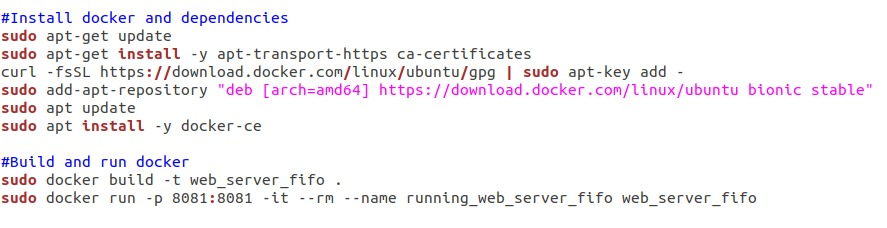
\includegraphics[width = \columnwidth]{installdocker.jpeg}
    \caption{Docker installer script.}
	\label{fig:installdocker}
\end{figure}

In contrast, to stop the docker container execution and uninstall it, the following script is executed.

\begin{figure}[H]
	\centering
	\captionsetup{justification=centering, margin=1cm}
    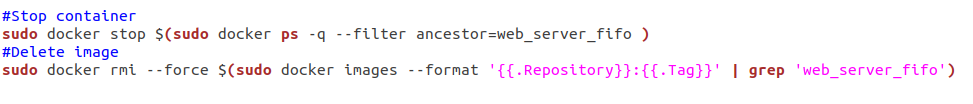
\includegraphics[width = \columnwidth]{removedocker.png}
    \caption{Docker uninstaller script.}
	\label{fig:removedocker}
\end{figure}

To create a daemon service within the docker it is necessary to create a script that contains the operations of starting, stopping, restarting and viewing the state of the daemon, which has the content shown in the following figure.

\begin{figure}[H]
	\centering
	\captionsetup{justification=centering, margin=1cm}
    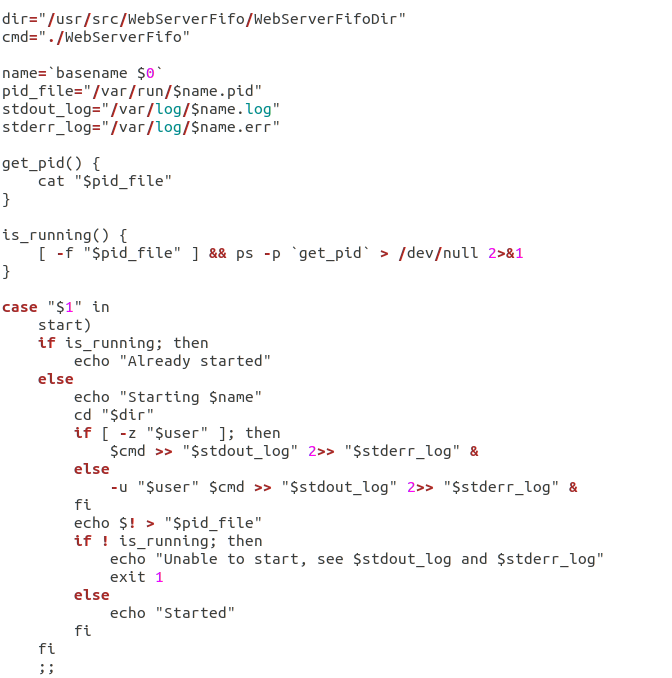
\includegraphics[width = \columnwidth]{installweb1.png}
    \caption{Web Server service installer script.}
	\label{fig:installweb1}
\end{figure}
\begin{figure}[H]
	\centering
	\captionsetup{justification=centering, margin=1cm}
    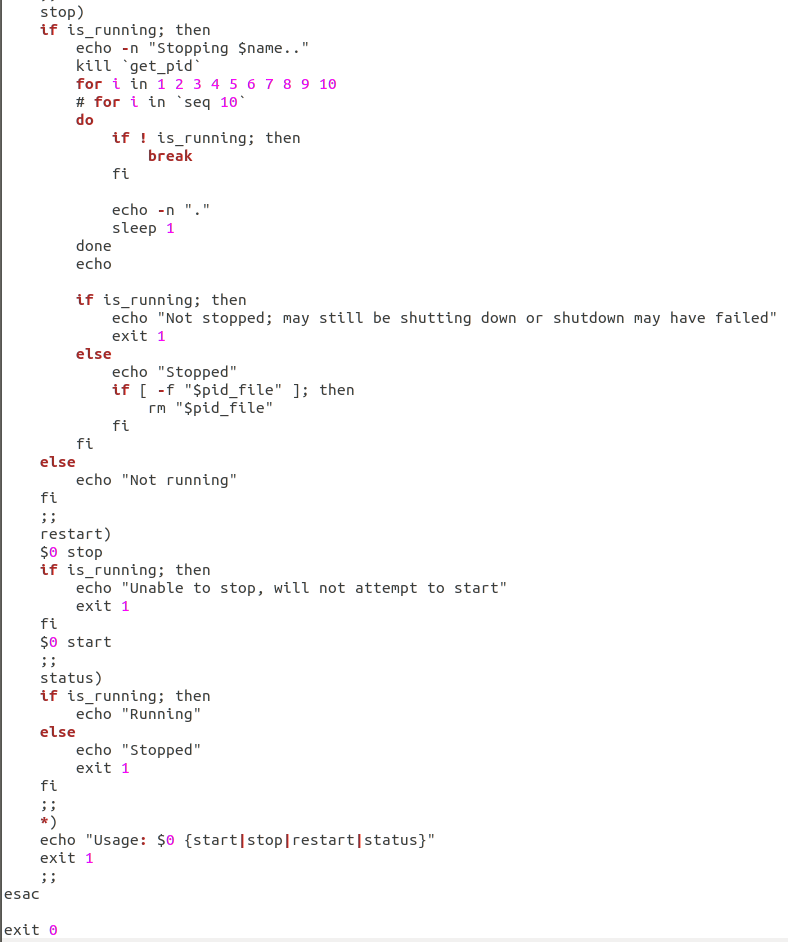
\includegraphics[width = \columnwidth]{installweb2.png}
    \caption{Web Server service installer script.}
	\label{fig:installweb2}
\end{figure}

The following script is used to stop and remove the web server daemon service. 

\begin{figure}[H]
	\centering
	\captionsetup{justification=centering, margin=1cm}
    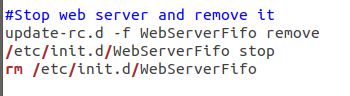
\includegraphics[width = 0.5\textwidth]{stopweb.png}
    \caption{Script to stop the web server daemon.}
	\label{fig:stopweb}
\end{figure}

As mentioned, what goes on in the environment inside a container is defined by a Dockerfile. For instance in this project the Dockerfile in the figure \ref{fig:docker}, were used.

\begin{figure}[H]
	\centering
	\captionsetup{justification=centering, margin=1cm}
    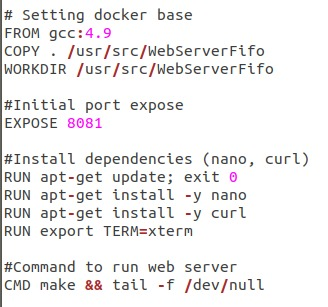
\includegraphics[width = 0.5\textwidth]{docker.jpeg}
    \caption{Dockerfile.}
	\label{fig:docker}
\end{figure}

In this file the environment inside the container is configured. First a gcc runtime environment is defined as the parent image, since the server application was implemented in C. The current directory contents are copied into the container at /usr/src/WebServerFifo, as well the working directory is set to the same directory.\\
The port 8081 is initially set available to the world outside this container. Then, all packages and dependencies needed are installed, and finally the Makefile is executed to perform the installation and configuration of the server when the container launches.\\
The Makefile content is presented in the figure \ref{fig:makefile}.

\begin{figure}[H]
	\centering
	\captionsetup{justification=centering, margin=1cm}
    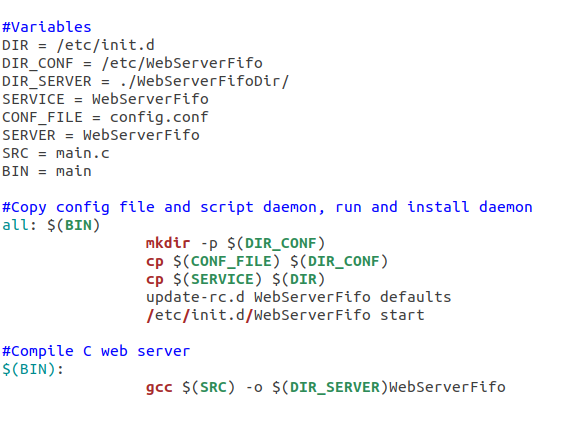
\includegraphics[width = 0.7\textwidth]{makefile.png}
    \caption{Makefile to install and configure the server.}
	\label{fig:makefile}
\end{figure}

The instructions in the Makefile are executed inside the docker container to install the web server. First the source code of this web server is compiled, generating a binary file located in /WebServerFifoDir in the current directory. Next the config file and the daemon script are copied to their respective folders and finally the daemon is installed and runned.\\

The web server has a main.c file that contains the functionality of it, based on \cite{Server}.
With the following methods:
\begin{enumerate}
    \item startServer: this method receives the port as input, it is responsible for lifting the web server, executing the socket and bind actions of the server, this using the sys / socket.h library.
    \item SendResponse: It receives as input the request to answer, it is responsible for verifying the request and responding using HTTP-1.1 for it, it executes methods such as recv to read the request and write to respond.
    \item main: Main method responsible for reading the values of configuration files, raise the server and keep listening and accepting connections using the other methods created.
    \item getLogPath: Method that reads the configuration file and returns the path for the file where to write the logs, for it looks for the line that has the value of "LOGFILE", in case of not finding the value of the path it returns the value for defect /var/log/syslog. Use methods such as fopen to open the file, fgets to read lines from the file, and sscanf to find the correct line.
    \item getPort: Method that reads the configuration file and returns the port to use, for it looks for the line that has the value of "PORT", in case of not finding the value of the port it returns the default value 8081. It uses methods as fopen to open the file, fgets to read lines from the file and sscanf to find the correct line.
    \item write: Receive the data to write and the path of the file to write, in addition to writing the required message write the time of the system to have a better log of the activity. Use the time.h library to get the time and methods such as open to open the file and write to write to it.
\end{enumerate}


\subsection{Benchmark tool}
The benchmark tool to develop is an application that will take the console parameters ($<$machine$>$ $<$port$>$ $<$file$>$r $<$N-threads$>$ $<$N-cycles$>$) and interpret them to create N number of threads with the mylpthread library where each one of these threads will open a connection socket to the server of the specified machine, each of these sockets will make the corresponding request the specified number of times. A general diagram is presented in the figure \ref{fig:BenchMarkDiagram} of how the benchmark tool works\\
\begin{figure}[H]
	\centering
	\captionsetup{justification=centering, margin=1cm}
    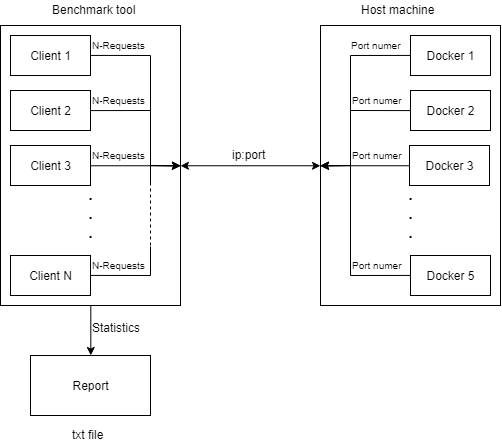
\includegraphics[width=\columnwidth]{BenchMarkDiagram.png}
    \caption{Benchmarck diagram.}
	\label{fig:BenchMarkDiagram}
\end{figure}
Each thread created for the requests will be in charge of storing the information of the corresponding times, that is, the average response time of the server in each request of the N cycles carried out. The time at which each of the cycles began to run will also be saved.\\
At the end of the test, general statistics of the result will be saved, such as: the date on which it was performed, the type of test (depending on the type of server), the IP address and port of the server, the number of requests made, the type of file that was requested, the size of the file, the total seconds that the test took and the average response time of all requests made. Figure \ref{fig:benchReportExamp} shows an example of the format that the test report will have.

\begin{figure}[H]
	\centering
	\captionsetup{justification=centering, margin=1cm}
    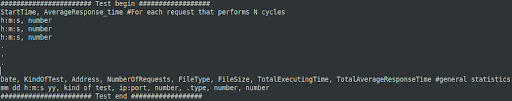
\includegraphics[width=\columnwidth]{images/benchReportExamp.png}
    \caption{Benchmarck report example.}
	\label{fig:benchReportExamp}
\end{figure}

\section{Instructions of how to use the programs}

\subsection{Installation and use of fifo web server}
\subsubsection{Requirements}
\begin{itemize}
    \item Work with Ubuntu (tested on a azure VM with Ubuntu 18.04).
\end{itemize}

\subsubsection{Creation and execution of the docker}
To create the docker it is only necessary to execute command: sh InstallDockerFifo.sh in the path where the delivered files are located, this is responsible for installing docker in the machine, do the docker build and execute it. It is necessary to add nano and curl to the docker, for that reason the installation commands are added to the docker, but when executing them some messages in red of some things that are not found are shown, however, this does not interfere in the correct functioning of the docker.

\subsubsection{Docker execution test}
When executing the previous command, the docker remains running. By default it is ready to run on port 8080, so to do tests it would only be necessary to go to a browser and make requests. Currently there are several test files in the directory of the web server (/usr/src/WebServerFifo/WebServerFifoDir), so the possible requests would be:\\
\centerline{http://server:8081/test.png}
\centerline{http://server:8081/test.pdf}
\centerline{http://server:8081/test.html}
\centerline{http://server:8081/test.bin}
\centerline{http://server:8081/test.mp4}
		
\subsubsection{Modify web server config and operations with the daemon}
To enter the running docker you must open another terminal and execute the command:\\
\centerline{sudo docker exec -it running\_web\_server\_fifo bash}

To perform the requested operations (start, stop, restart, view status) of the web server, as well as modify the configuration file, the following commands must be executed:

To perform actions on the daemon:\\
\centerline{Start daemon: /etc/init.d/WebServerFifo start}
\centerline{Stop daemon: /etc/init.d/WebServerFifo stop}
\centerline{Restart daemon: /etc/init.d/WebServerFifo restart}
\centerline{Daemon status: /etc/init.d/WebServerFifo status}

To modify the configuration file\\
\centerline{--nano /etc/WebServerFifo/config.conf}
\subsubsection{Uninstall docker}
To uninstall the docker it is necessary to execute the command: sh RemoveDockerFifo.sh in the path where the delivered files are located

\section{Student activity log}

\begin{table}[H]
\centering
\caption{Bryan Abarca Activity Log}
\begin{tabular}{|p{7cm}|p{7cm}|}
\hline
\textbf{Activity} & \textbf{Duration} \\ \hline
Reading and analysis of the project specification. & 1 h \\ \hline
Research on the operation and use of docker containers. & 2 h\\ \hline
Implementation of the docker container and and adjustments in the makefile. & 6 h\\ \hline
Documentation. & 3 h\\ \hline
Total & 12 h\\ \hline
\end{tabular}
\end{table}

\begin{table}[H]
\centering
\caption{Raúl Arias Activity Log}
\begin{tabular}{|p{7cm}|p{7cm}|}
\hline
\textbf{Activity} & \textbf{Duration} \\ \hline
Reading and analysis of the project specification. & 1 h \\ \hline 
Error correction of FIFO web server (logs, makefile, uninstall file). & 4 h  \\ \hline
Research on the operation and use of docker containers. & 2 h \\ \hline
Support in the creation of the docker. & 2 h \\ \hline
Implementation of the daemon for SysV. & 2 h \\ \hline
Documentation. & 2 h\\ \hline
Total & 13 h \\ \hline
\end{tabular}
\end{table}

\begin{table}[H]
\centering
\caption{Rony Paniagua Activity Log}
\begin{tabular}{|p{7cm}|p{7cm}|}
\hline
\textbf{Activity} & \textbf{Duration} \\ \hline
Reading and analysis of the project specification. & 1 h \\ \hline
High level design of the benchmark. & 3 h\\ \hline
Research on the operation and use of docker containers. & 2 h\\ \hline
Implementation of the installation and destruction script of the docker container. & 2 h\\ \hline
Documentation. & 3 h\\ \hline
Total & 11 h\\ \hline
\end{tabular}
\end{table}

\section{Project final status}
So far we have the successful implementation of the docker that contains the fifo web server which works correctly without errors detected.
\section{Conclusions}
The use of dockers presents a series of advantages such as the compatibility that allows to execute applications independently of the platform in which they are being executed, besides it allows to realize a standardization and simplicity of configurations, all the previous allows the deploy of applications to be much easier and faster regardless of the platform used.
\section{Suggestions}
It is recommended to start with images of dockers that have installed some of the components that are needed, for example the start of the docker from gcc avoids having to add the commands necessary for the installation of gcc
\section{References}
\begin{thebibliography}{1}

\bibitem{WhatDocker}
Docker. [Online]. Available in: https://www.docker.com/resources/what-container

\bibitem{DockerEngine}
Docker. [Online]. Available in: https://www.docker.com/products/docker-engine

\bibitem{DockerContainer}
docker docs. Get started, part 2: Containers. [Online]. Available in: https://docs.docker.com/get-started/part2/

\bibitem{Server}
Rastogi, A. (2010). A Very Simple HTTP Server writen in C. [Online]
Abhijeet’s Blog. Available in: https://blog.abhijeetr.com/2010/04/very-
simple-http-server-writen-in-c.html.


\end{thebibliography}

\end{document}
